\documentclass[12pt, letterpaper]{article}
\usepackage[T1]{fontenc}
\usepackage{amsmath}
\usepackage{graphicx}  

\title{Metody Numeryczne - Projekt 1:\newline Wskaznik MACD}
\author{Jakub Szymczyk, 198134}
\date{Marzec 2025}
\begin{document}
\maketitle

\section{Wstep}
\par
Głównym celem projektu była implementacja wskaźnika MACD oraz analiza jego przydatności w automatycznym podejmowaniu decyzji o kupnie lub sprzedaży akcji.
\bigskip
\par Analiza wskaźnika została przeprowadzona na notowaniach indeksu giełdowego S\&P 500 oraz kursie Bitcoina.
\bigskip
\par Projekt został zrealizowany w języku Python z wykorzystaniem bibliotek pandas, numpy oraz matplotlib. Biblioteki te służyły jedynie do wczytywania danych oraz wizualizacji wyników, natomiast wszystkie obliczenia zostały zaimplementowane bezpośrednio w kodzie źródłowym projektu.
\section{Czym jest MACD}
Wskaźnik MACD (\textit{Moving Average Convergence/Divergence}) został opracowany przez Gerarda Appela w 1979 roku i stanowi jedno z najpopularniejszych narzędzi analizy technicznej. Jego głównym celem jest identyfikacja trendów rynkowych poprzez analizę zbieżności i rozbieżności dwóch średnich wykładniczych (EMA – \textit{Exponential Moving Average}).

\bigskip
Wskaźnik MACD obliczany jest jako różnica wartości krótkoterminowej i długoterminowej średniej wykładniczej, najczęściej z okresami 12 i 26 dni. Dodatkowo, na wykresie często uwzględnia się tzw. linię sygnałową, będącą 9-okresową średnią wykładniczą wartości MACD, która pomaga w interpretacji sygnałów kupna i sprzedaży.

\bigskip
Podstawowe zasady interpretacji wskaźnika MACD obejmują:
\begin{itemize}
\item \textbf{Przecięcie linii MACD i linii sygnałowej} – sygnał kupna pojawia się, gdy MACD przecina linię sygnałową od dołu, natomiast sygnał sprzedaży – gdy przecina ją od góry.
\item \textbf{Przecięcie poziomu zerowego} – gdy MACD przechodzi powyżej zera, wskazuje na rosnącą siłę trendu wzrostowego, a gdy spada poniżej zera, może sygnalizować początek trendu spadkowego.
\item \textbf{Dywergencje} – jeśli cena akcji lub indeksu osiąga nowe szczyty, ale MACD nie potwierdza tego wzrostu, może to wskazywać na osłabienie trendu i potencjalną zmianę kierunku.
\end{itemize}

\bigskip
Dzięki swojej konstrukcji wskaźnik MACD jest często wykorzystywany w strategiach automatycznego handlu oraz analizie algorytmicznej.

\section{Implementacja}

Wskaźnik MACD został zaimplementowany w następujący sposób:
\begin{equation}
    MACD = EMA_{12} - EMA_{26}
\end{equation}
\begin{equation}
    SIGNAL = EMA_9(MACD)
\end{equation}

gdzie $EMA_N$ oznacza wykładniczą średnią kroczącą (ang. \textit{Exponential Moving Average}) obliczaną według wzoru:
\begin{equation}
    EMA_N^{today} = (p \cdot \alpha) + EMA_N^{yesterday} \cdot (1 - \alpha)
\end{equation}

gdzie:
\begin{itemize}
    \item $p$ – cena zamknięcia w danym przedziale czasowym,
    \item $\alpha$ – współczynnik wygładzający, określony jako:
    \begin{equation}
        \alpha = \frac{2}{N+1}
    \end{equation}
    \item $N$ – liczba okresów.
\end{itemize}

Który został wyprowadzony z:
\begin{equation}
    EMA_N(i) = \frac{x_i + (1 - \alpha)x_{i-1} + (1 - \alpha)^2 x_{i-2} + \dots + (1 - \alpha)^i x_0}
    {1 + (1 - \alpha) + (1 - \alpha)^2 + \dots + (1 - \alpha)^i}
\end{equation}

\section{Dane}

\section{Implementacja wskaźnika MACD}

Wskaźnik MACD został zaimplementowany w następujący sposób:
\begin{equation}
    MACD = EMA_{12} - EMA_{26}
\end{equation}
\begin{equation}
    SIGNAL = EMA_9(MACD)
\end{equation}

gdzie $EMA_N$ oznacza wykładniczą średnią kroczącą (ang. \textit{Exponential Moving Average}) obliczaną według wzoru:
\begin{equation}
    EMA_N^{today} = (p \cdot \alpha) + EMA_N^{yesterday} \cdot (1 - \alpha)
\end{equation}

gdzie:
\begin{itemize}
    \item $p$ – cena zamknięcia w danym przedziale czasowym,
    \item $\alpha$ – współczynnik wygładzający, określony jako:
    \begin{equation}
        \alpha = \frac{2}{N+1}
    \end{equation}
    \item $N$ – liczba okresów.
\end{itemize}

Który został wyprowadzony z:
\begin{equation}
    EMA_N(i) = \frac{x_i + (1 - \alpha)x_{i-1} + (1 - \alpha)^2 x_{i-2} + \dots + (1 - \alpha)^i x_0}
    {1 + (1 - \alpha) + (1 - \alpha)^2 + \dots + (1 - \alpha)^i}
\end{equation}

\section{Dane do analizy}

Do analizy wykorzystujemy notowania dwóch instrumentów finansowych:

\subsection{Indeks giełdowy S\&P 500}
Analizujemy indeks S\&P 500 w okresie od końca 2014 do końca 2024. Jest to indeks, na którym bazuje wiele funduszy ETF, co umożliwia nam ogólną analizę skuteczności działania wskaźnika MACD. 

\begin{figure}[h!]
    \centering
    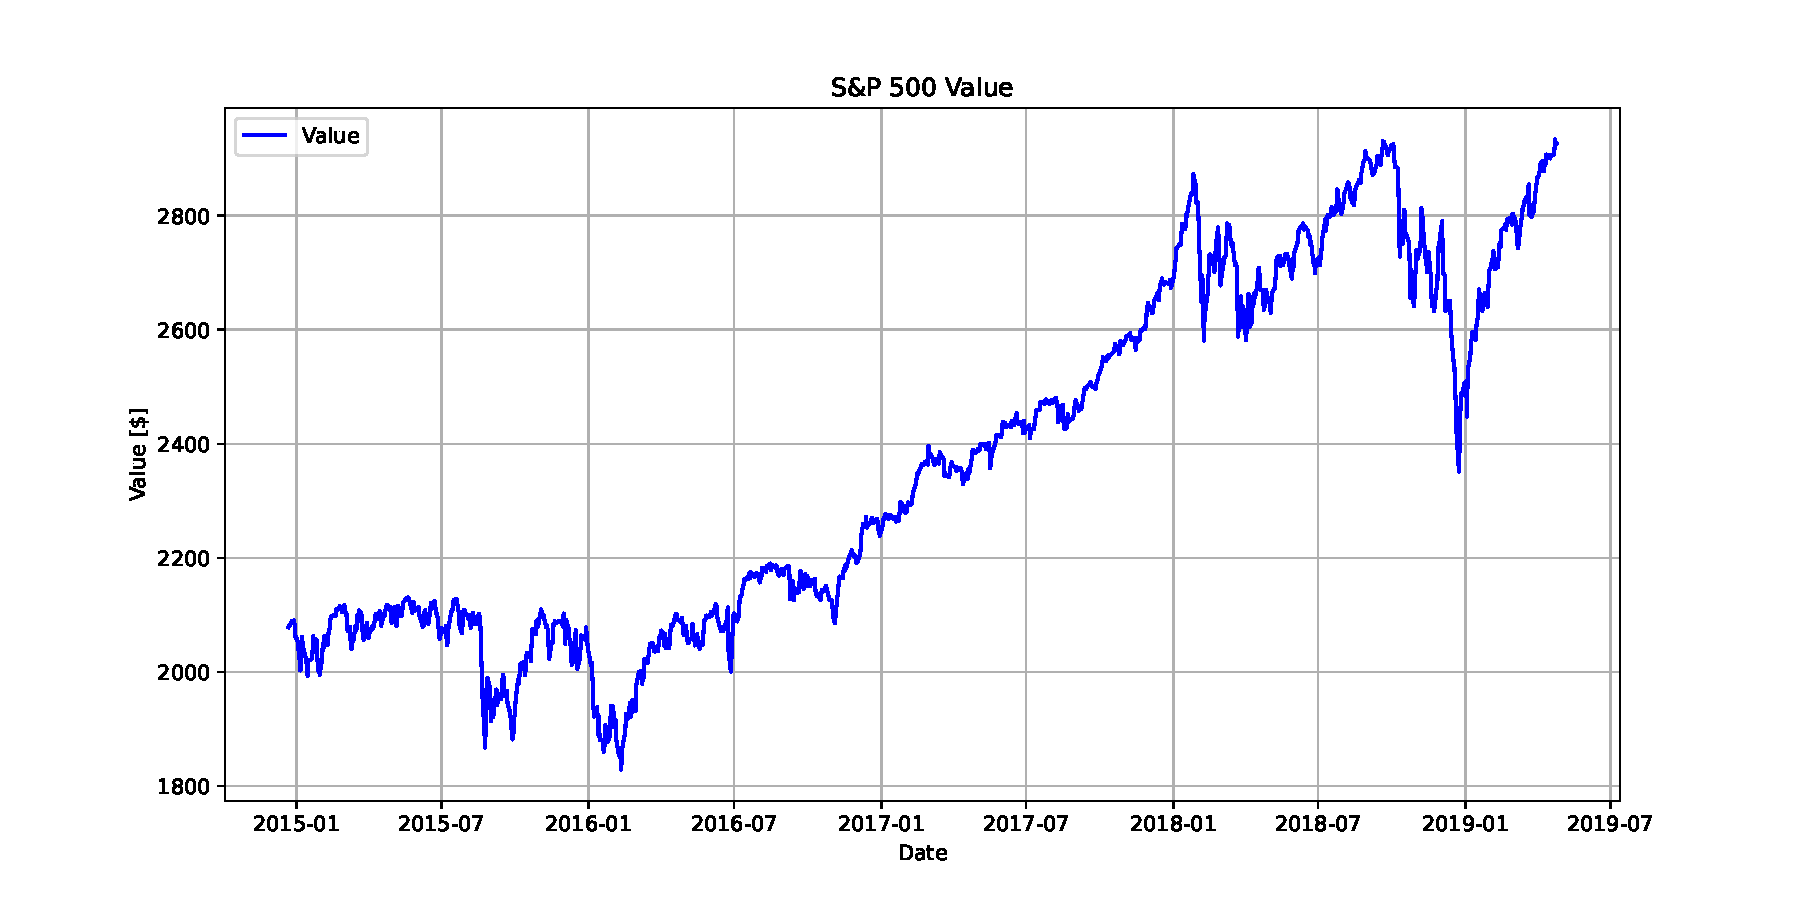
\includegraphics[width=\linewidth]{wykres S&P 500 from 0.pdf}
    \caption{Wykres indeksu S\&P 500 od roku 2014 do 2017}
    \label{fig:sp500_2014_2017}
\end{figure}

\vspace{-1cm}  % Zmniejszamy przestrzeń, żeby tekst był bliżej wykresu

\begin{figure}[h!]
    \centering
    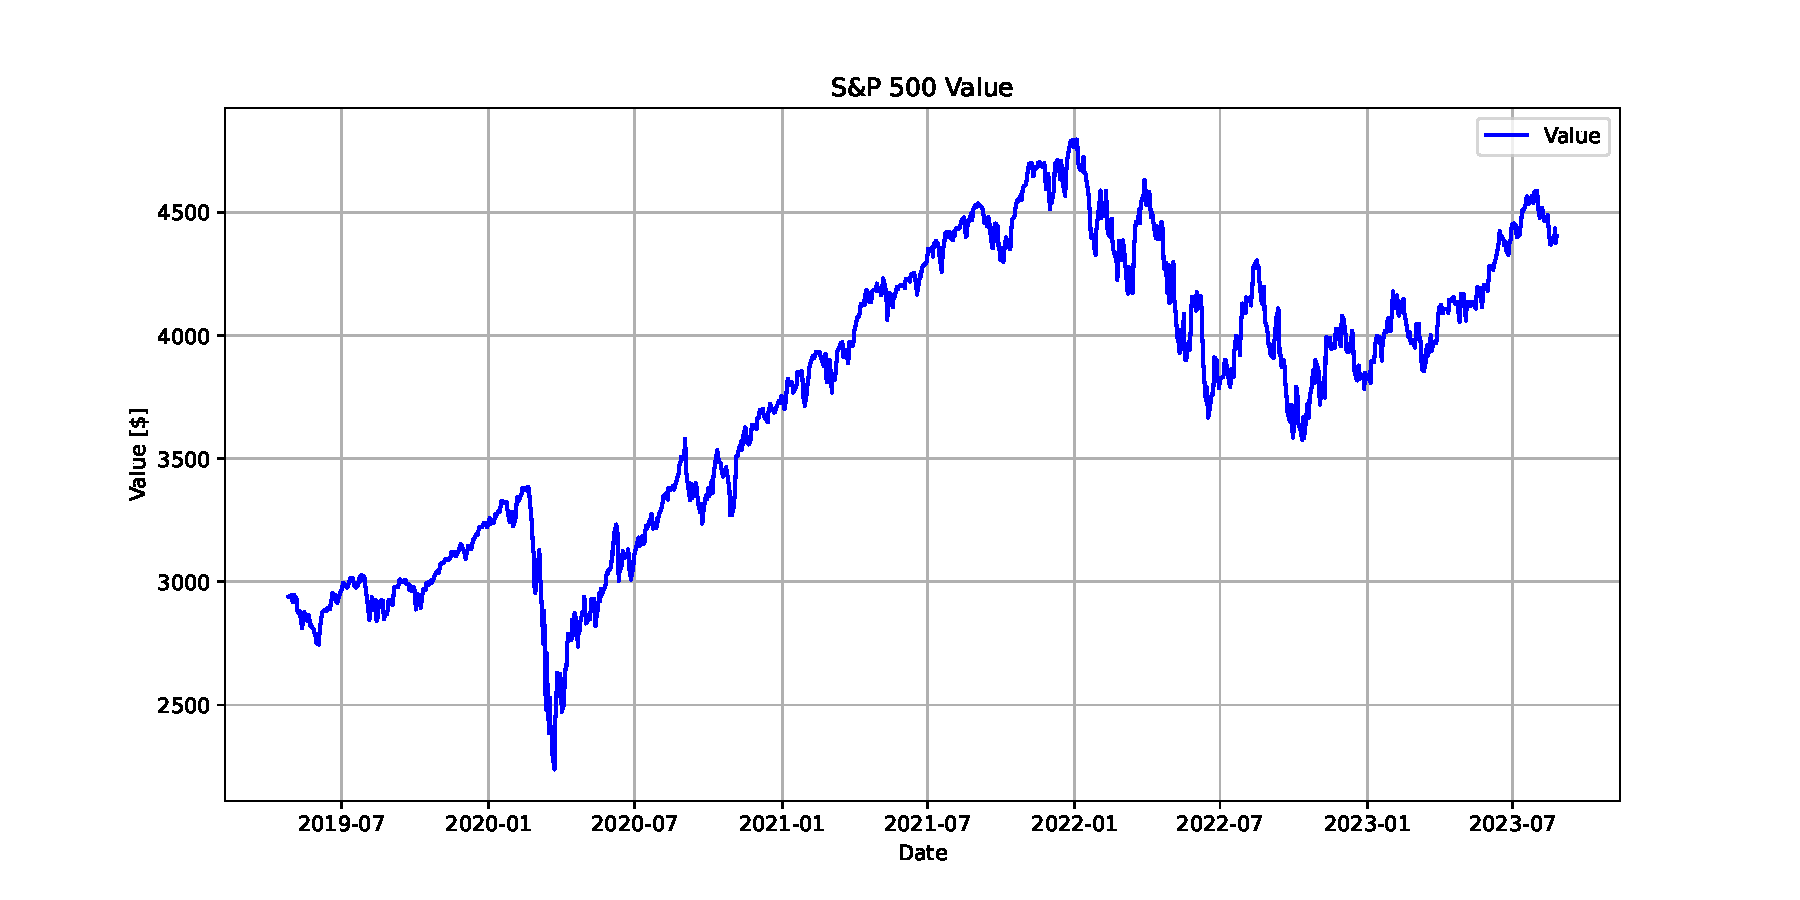
\includegraphics[width=\linewidth]{wykres S&P 500 from 3.pdf}
    \caption{Wykres indeksu S\&P 500 od roku 2019 do 2023}
    \label{fig:sp500_2019_2023}
\end{figure}

\subsection{Kryptowaluta Bitcoin}
Analizujemy notowania Bitcoina w okresie od końca 2014 do 2022. Ten instrument pozwala na przetestowanie wskaźnika MACD w bardzo zmiennych warunkach rynkowych.

\begin{figure}[h!]
    \centering
    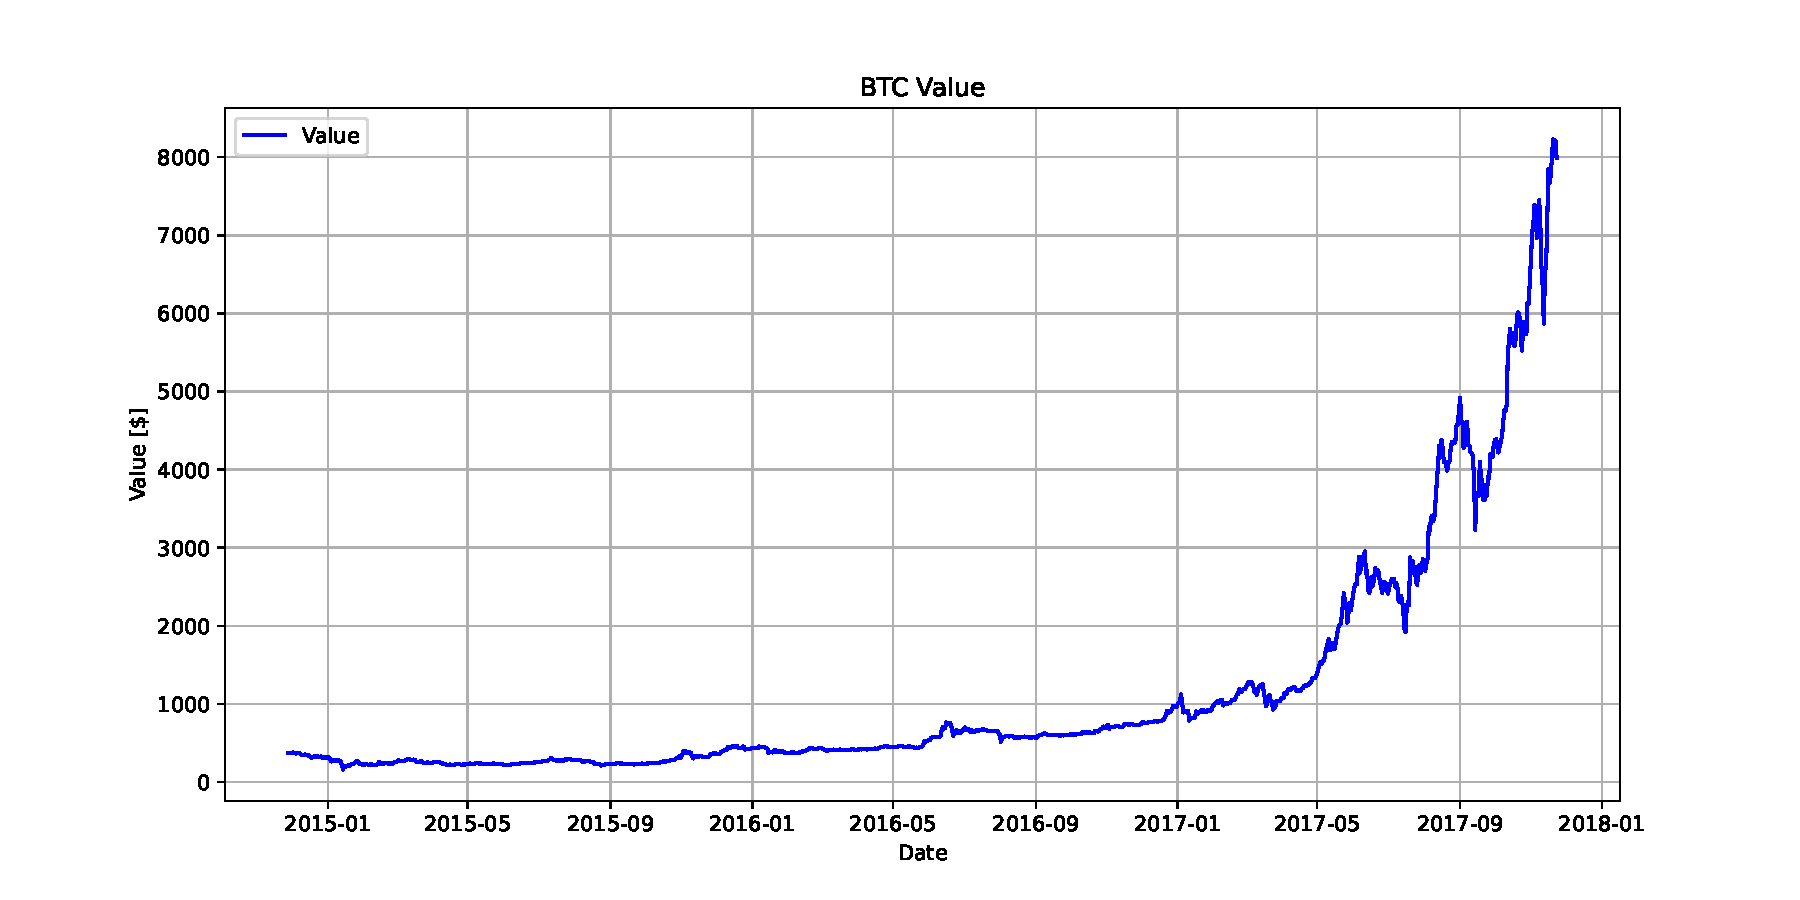
\includegraphics[width=\linewidth+0.4]{wykres BTC from 0.pdf}
    \caption{Wykres wartości BTC od roku 2014 do 2017}
    \label{fig:btc_2014_2017}
\end{figure}

\section{Relacja MACD do danych wejsciowych}

\subsection{S\&P 500 2014-2019}
\begin{figure}[h!]
    \centering
    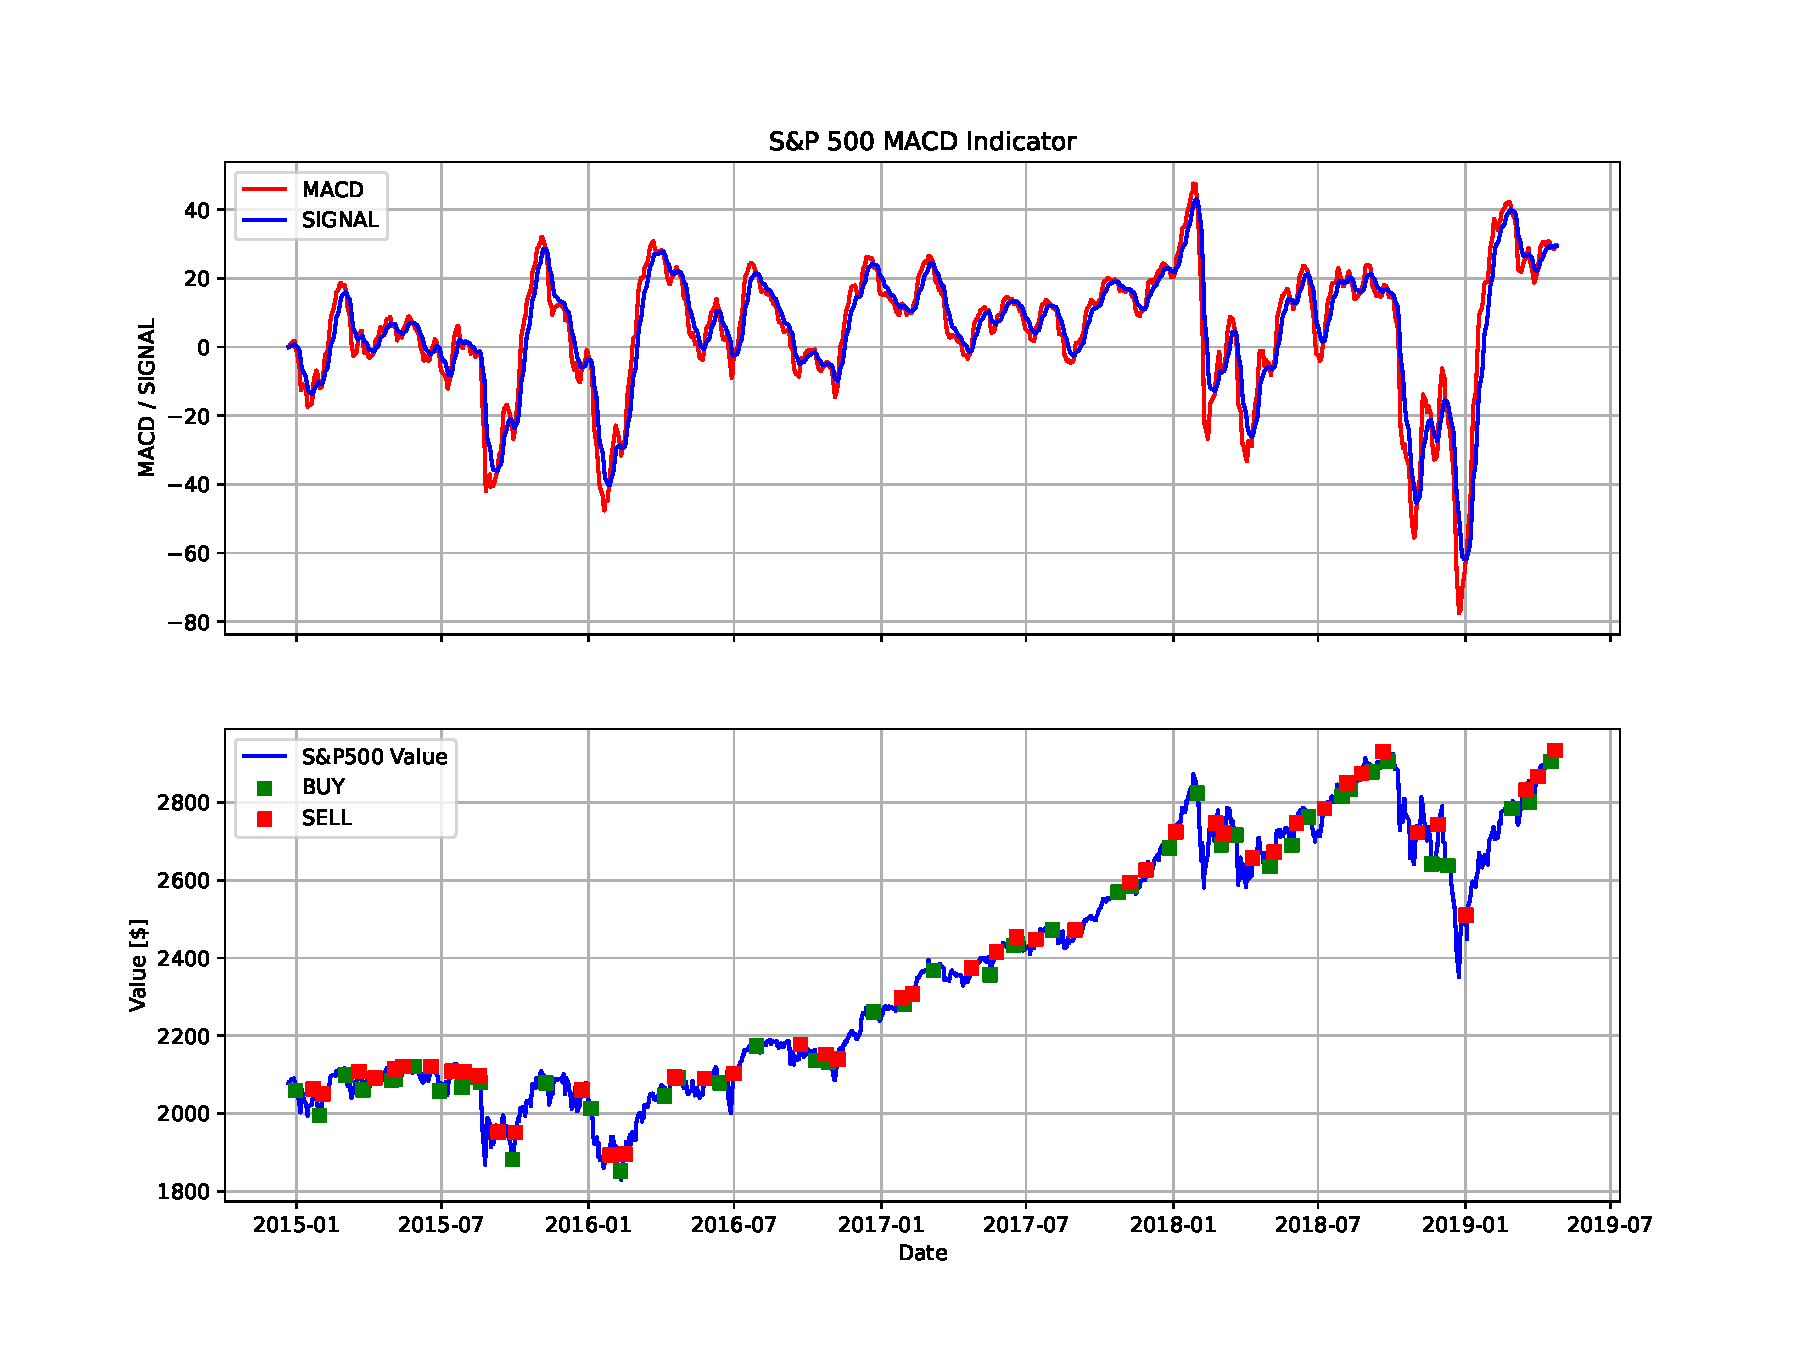
\includegraphics[width=\linewidth]{MACD S&P500 from 0.pdf}
    \caption{Wykresy wartosci oraz wskaznika MACD dla S\&P 500 2014-2019}
    \label{fig:sp500_2014_2017}
\end{figure}

\begin{itemize}
\item Sygnały \textbf{BUY} występowały na początku wzrostowych trendów, co pozwalało na korzystne wejście na rynek. Sygnały \textbf{SELL} zazwyczaj skutecznie wskazywały na momenty osłabienia trendu wzrostowego lub rozpoczęcia spadków.
\item Przecięcie poziomu zerowego w górę potwierdzało wzrostową dynamikę rynku, a spadek poniżej tego poziomu zapowiadał tendencję spadkową.
\end{itemize}

\vspace{5cm}  % Zmniejszamy przestrzeń, żeby tekst był bliżej wykresu
\subsection{S\&P 500 2019-2023}
\begin{figure}[h!]
    \centering
    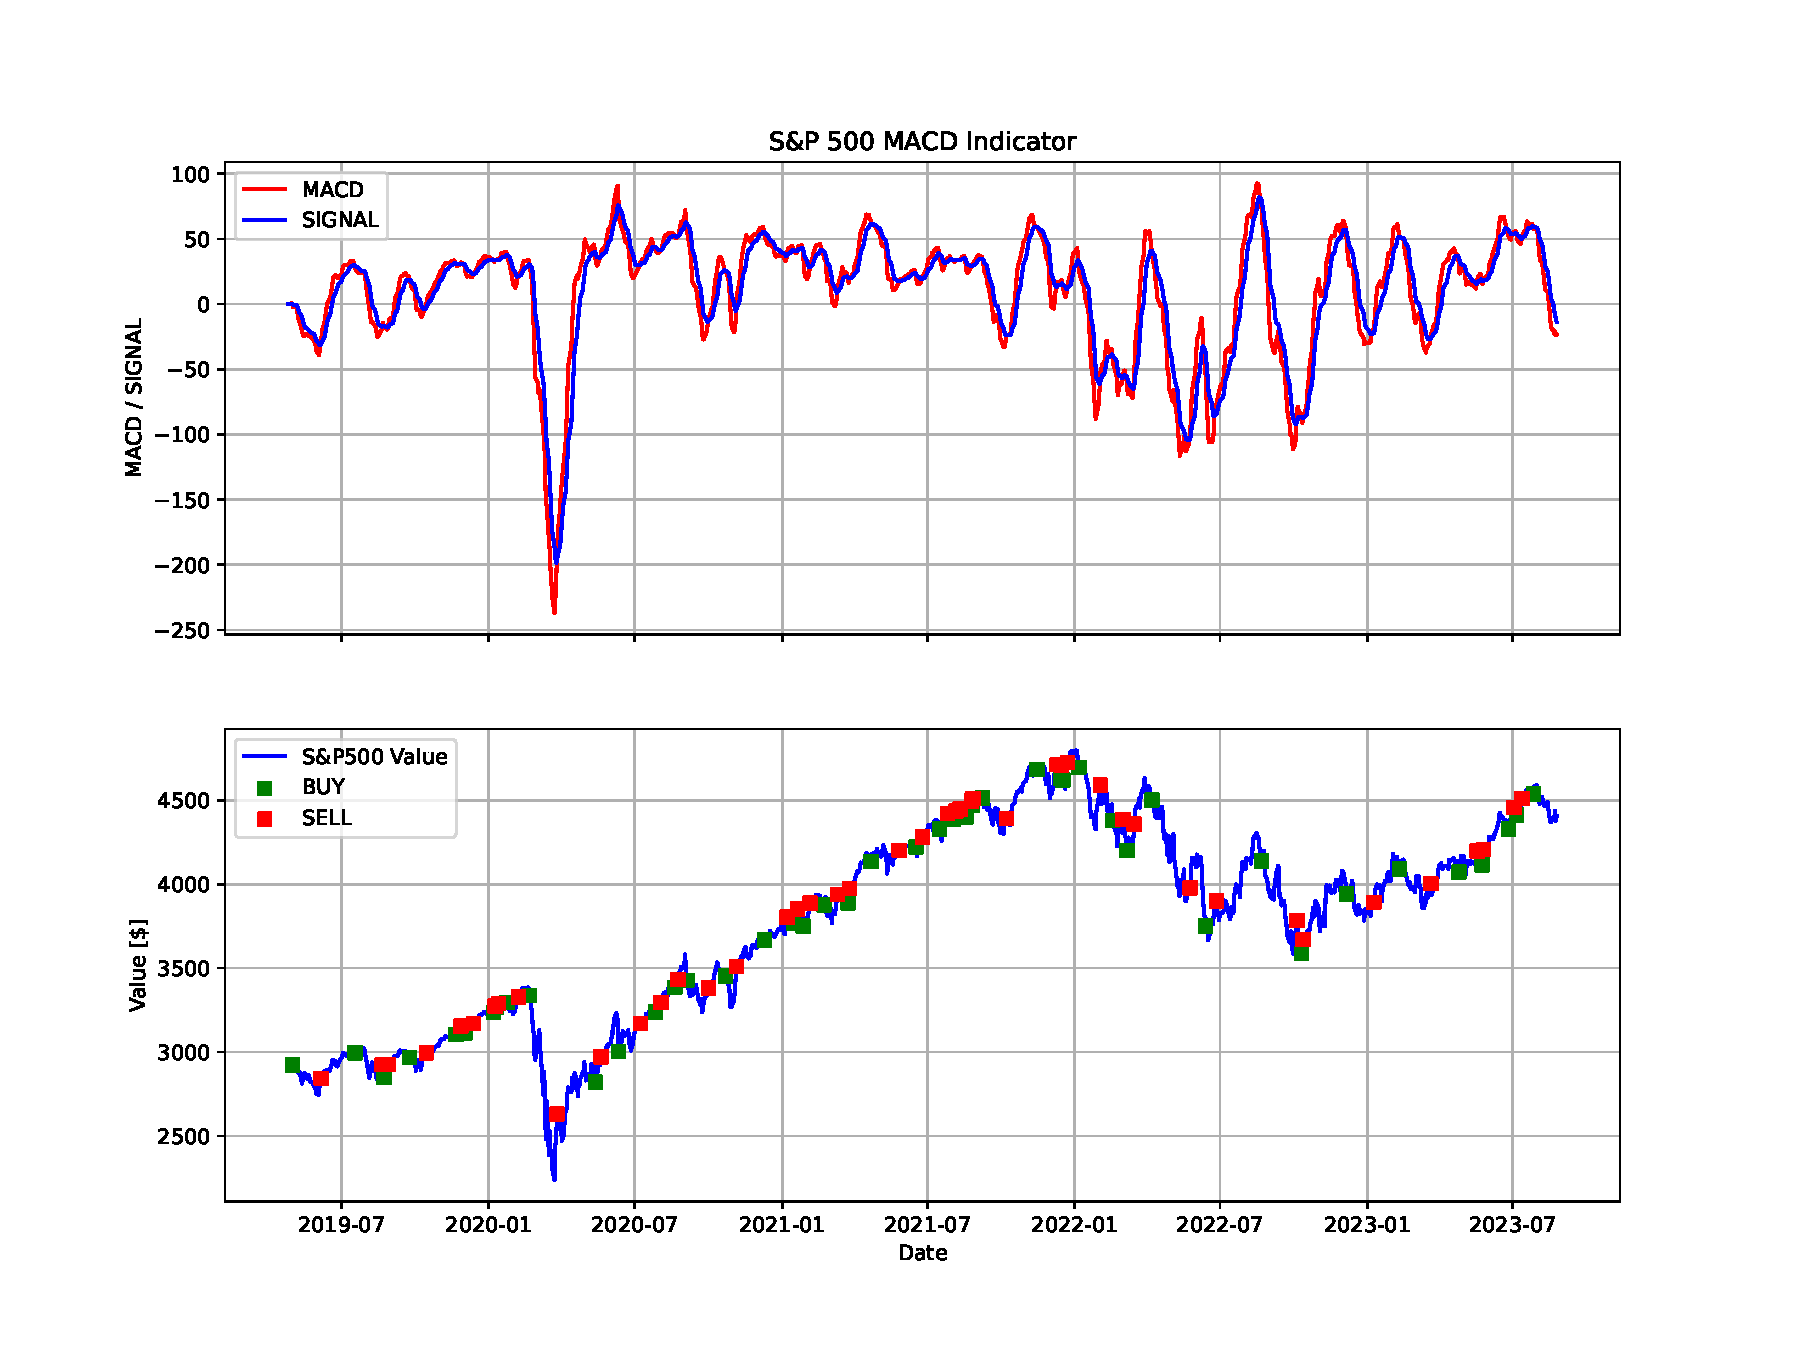
\includegraphics[width=\linewidth]{MACD S&P500 from 3.pdf}
    \caption{Wykresy wartosci oraz wskaznika MACD dla S\&P 500 2019-2023} 
    \label{fig:sp500_2019_2023}
\end{figure}

\begin{itemize}
\item W tym okresie MACD dobrze identyfikował zarówno krótkoterminowe korekty, jak i długotrwałe trendy.
\item Silne odchylenia MACD wskazywały na dynamiczne ruchy cenowe, co okazało się użyteczne w przewidywaniu okresów dużej zmienności.
\end{itemize}

\vspace{5cm}  % Zmniejszamy przestrzeń, żeby tekst był bliżej wykresu
\subsection{BTC 2014-2019}
\begin{figure}[h!]
    \centering
    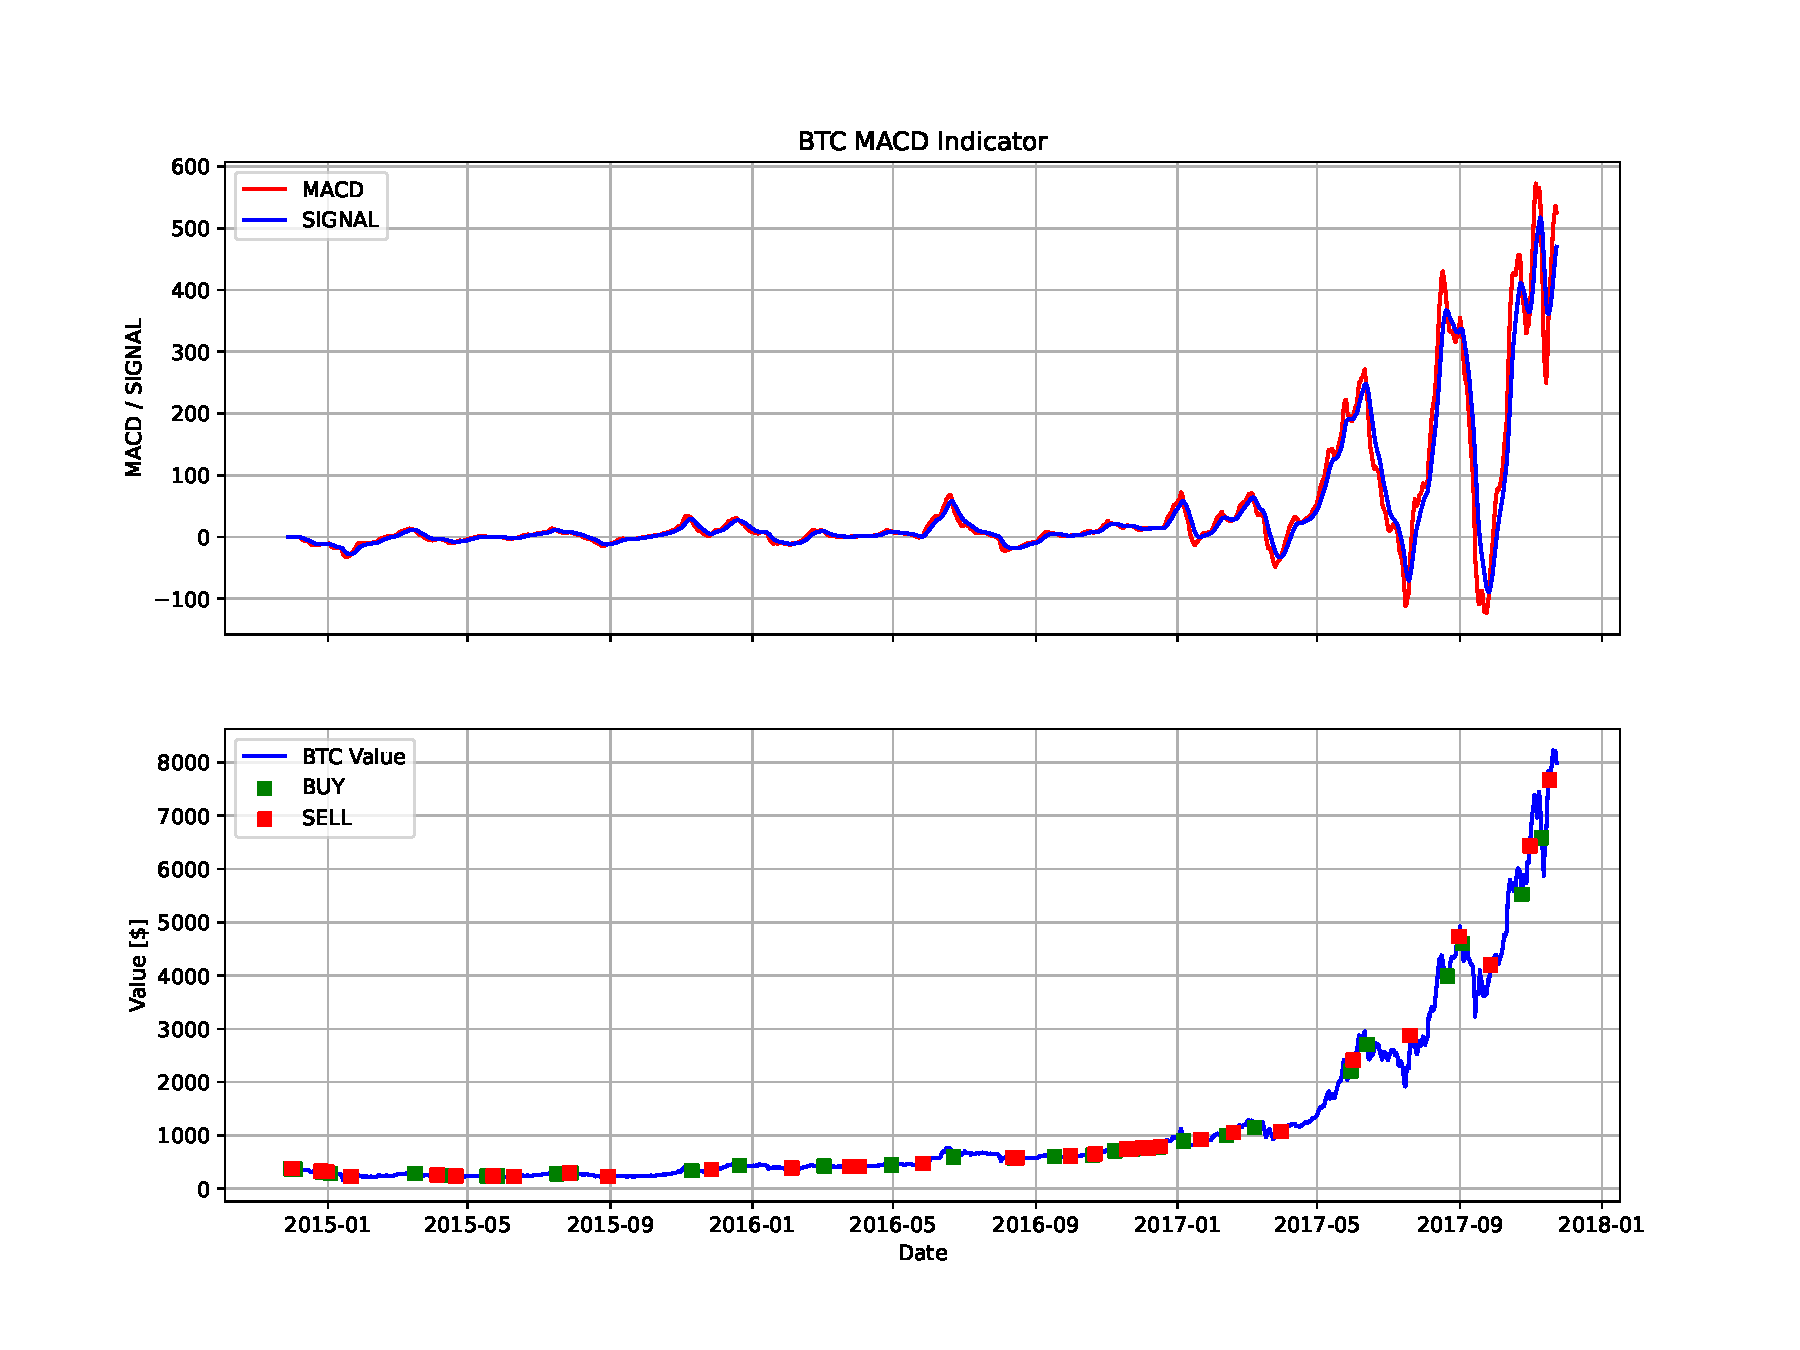
\includegraphics[width=\linewidth]{MACD BTC from 0.pdf}
    \caption{Wykresy wartosci oraz wskaznika MACD dla BTC 2014-2019}
    \label{fig:BTC_2014_2017}
\end{figure}

\subsection*{Bitcoin (2014-2019)}
\begin{itemize}
\item Sygnały \textbf{BUY} i \textbf{SELL} były mniej przewidywalne niż w przypadku indeksu S\&P 500, co wynika z większej zmienności rynku kryptowalut.
\item W okresach dynamicznych wzrostów MACD generował liczne sygnały, co wymagało dodatkowej analizy w celu uniknięcia fałszywych alarmów.
\end{itemize}


\vspace{5cm}  % Zmniejszamy przestrzeń, żeby tekst był bliżej wykresu
\subsection*{Podsumowanie}
Wskaźnik MACD wykazał się wysoką skutecznością w identyfikacji trendów na rynku S\&P 500, chociaz przy duzych zmianach na rynku sprawial powodowal wiecej falszy, a co gorsza czesto powodujacych duze straty. Natomiast w przypadku Bitcoina, z powodu jego wysokiej zmiennosci (ang. volitlity) mozemy zauwazyc ze  generował więcej fałszywych sygnałów, niz nawet w S\&P 500 .Połączenie MACD z dodatkowymi wskaźnikami technicznymi oraz analizą fundamentalną może znacząco zwiększyć trafność prognoz inwestycyjnych.

\end{document}